\section{Particle and bunch tracking}
\label{sec:tracking}

The bunch helpers accept rows in the Python/PyParticleBunch order \texttt{x, xp, y, yp, z, dE}; \texttt{dE} is a total-energy deviation. In the default PTC tracking state used by these helpers, the fifth coordinate is relative momentum deviation, \(\delta=p/p_0-1\), rather than relative energy deviation. With synchronous energy \(E_0=p_0c/\beta_0\) and inferred rest mass \(m^2=E_0^2-(p_0c)^2\), the wrapper computes \(\delta=\sqrt{(E_0+dE)^2-m^2}/p_0c-1\). The inverse is \(dE=\sqrt{m^2+[p_0c(1+\delta)]^2}-E_0\). The sixth-coordinate mapping is \(L=-z/\beta_0\). This documents the implemented convention and its code/manual basis; it is not a physics validation of every active PTC state or operating regime. [claim:TRACK-01] [claim:TRACK-02]

\path{track_bunch()} uses the same conversion at each node while updating the synchronous reference, and returns either the final array or one copied snapshot per turn when \texttt{record\_turns=True}. The low-level \path{track_particle_ptc()} and \path{track_particle_ptc_with_loss()} methods do not perform this conversion: they forward six raw PTC coordinates, whose meaning depends on the active PTC state. [claim:TRACK-03] [claim:TRACK-02]

The standard bunch example creates its input with the PyParticleBunch helper, tracks a fixed-size bunch for a stated turn count, and writes before/after diagnostic dashboards and CSV files. The outputs show an example run only; they do not prove model validity for other lattices or operating conditions. [claim:EXAMPLE-02]

\begin{figure}[ht]
  \centering
  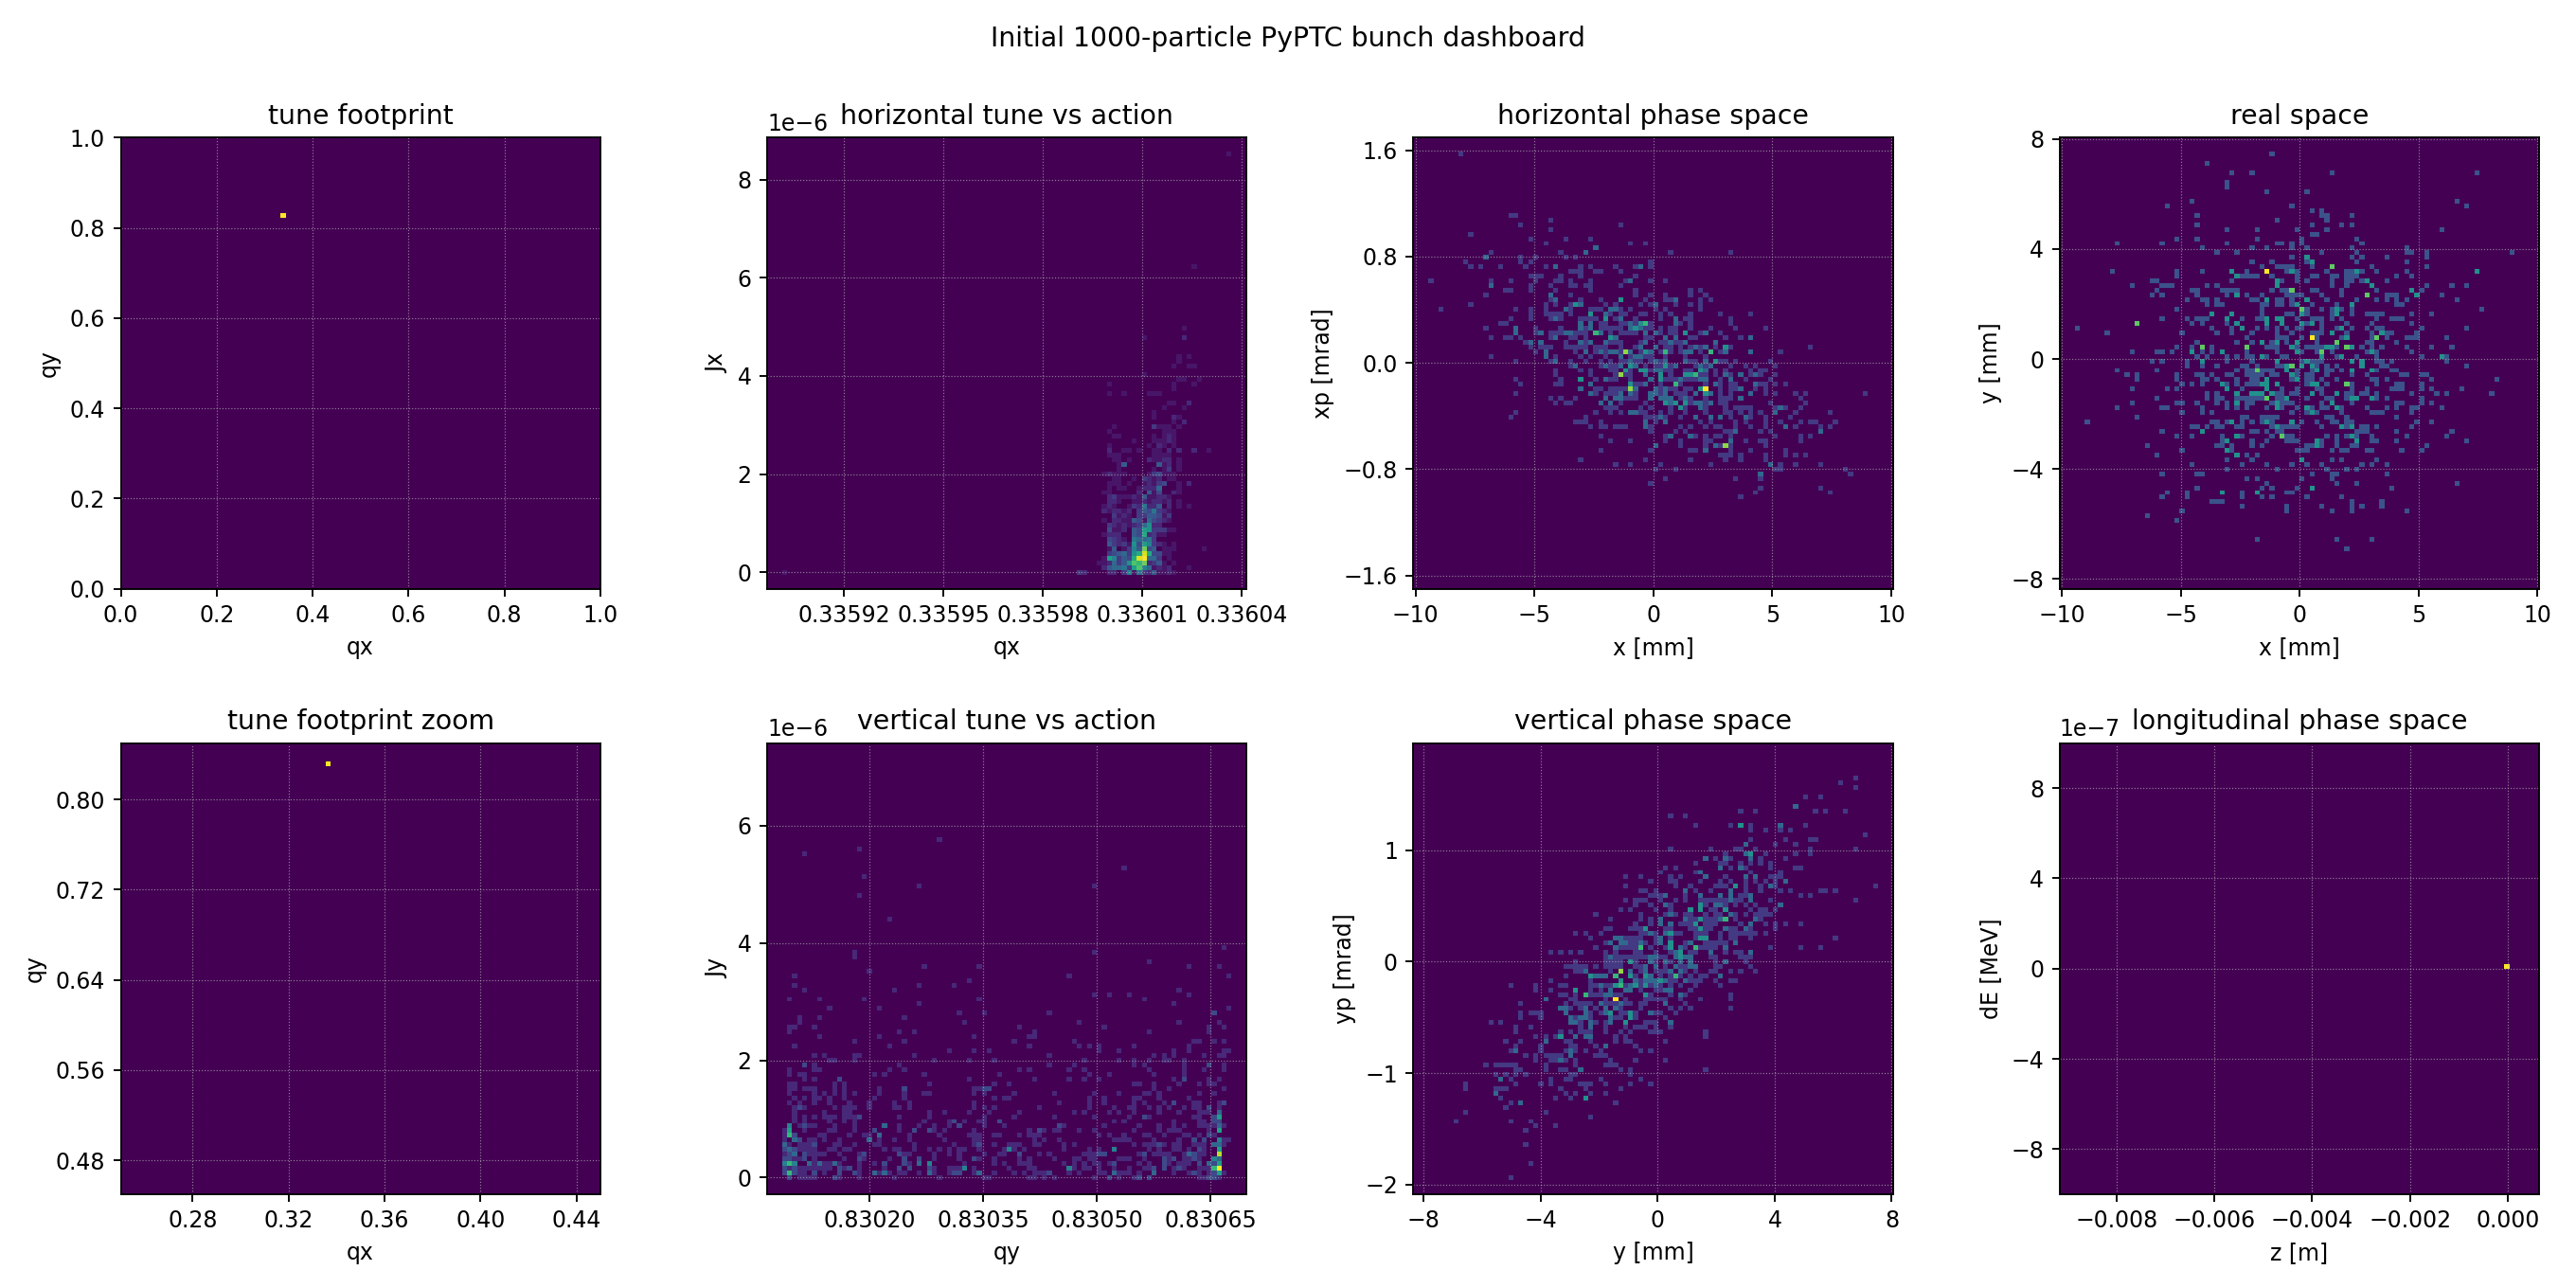
\includegraphics[width=0.88\textwidth]{figures/bunch_initial_dashboard.png}
  \caption{Initial bunch dashboard copied from the standard bunch example output. It records the available diagnostic view before tracking; the associated output directory contains the run summary and diagnostic data. [claim:PROV-03]}
\end{figure}

\begin{figure}[ht]
  \centering
  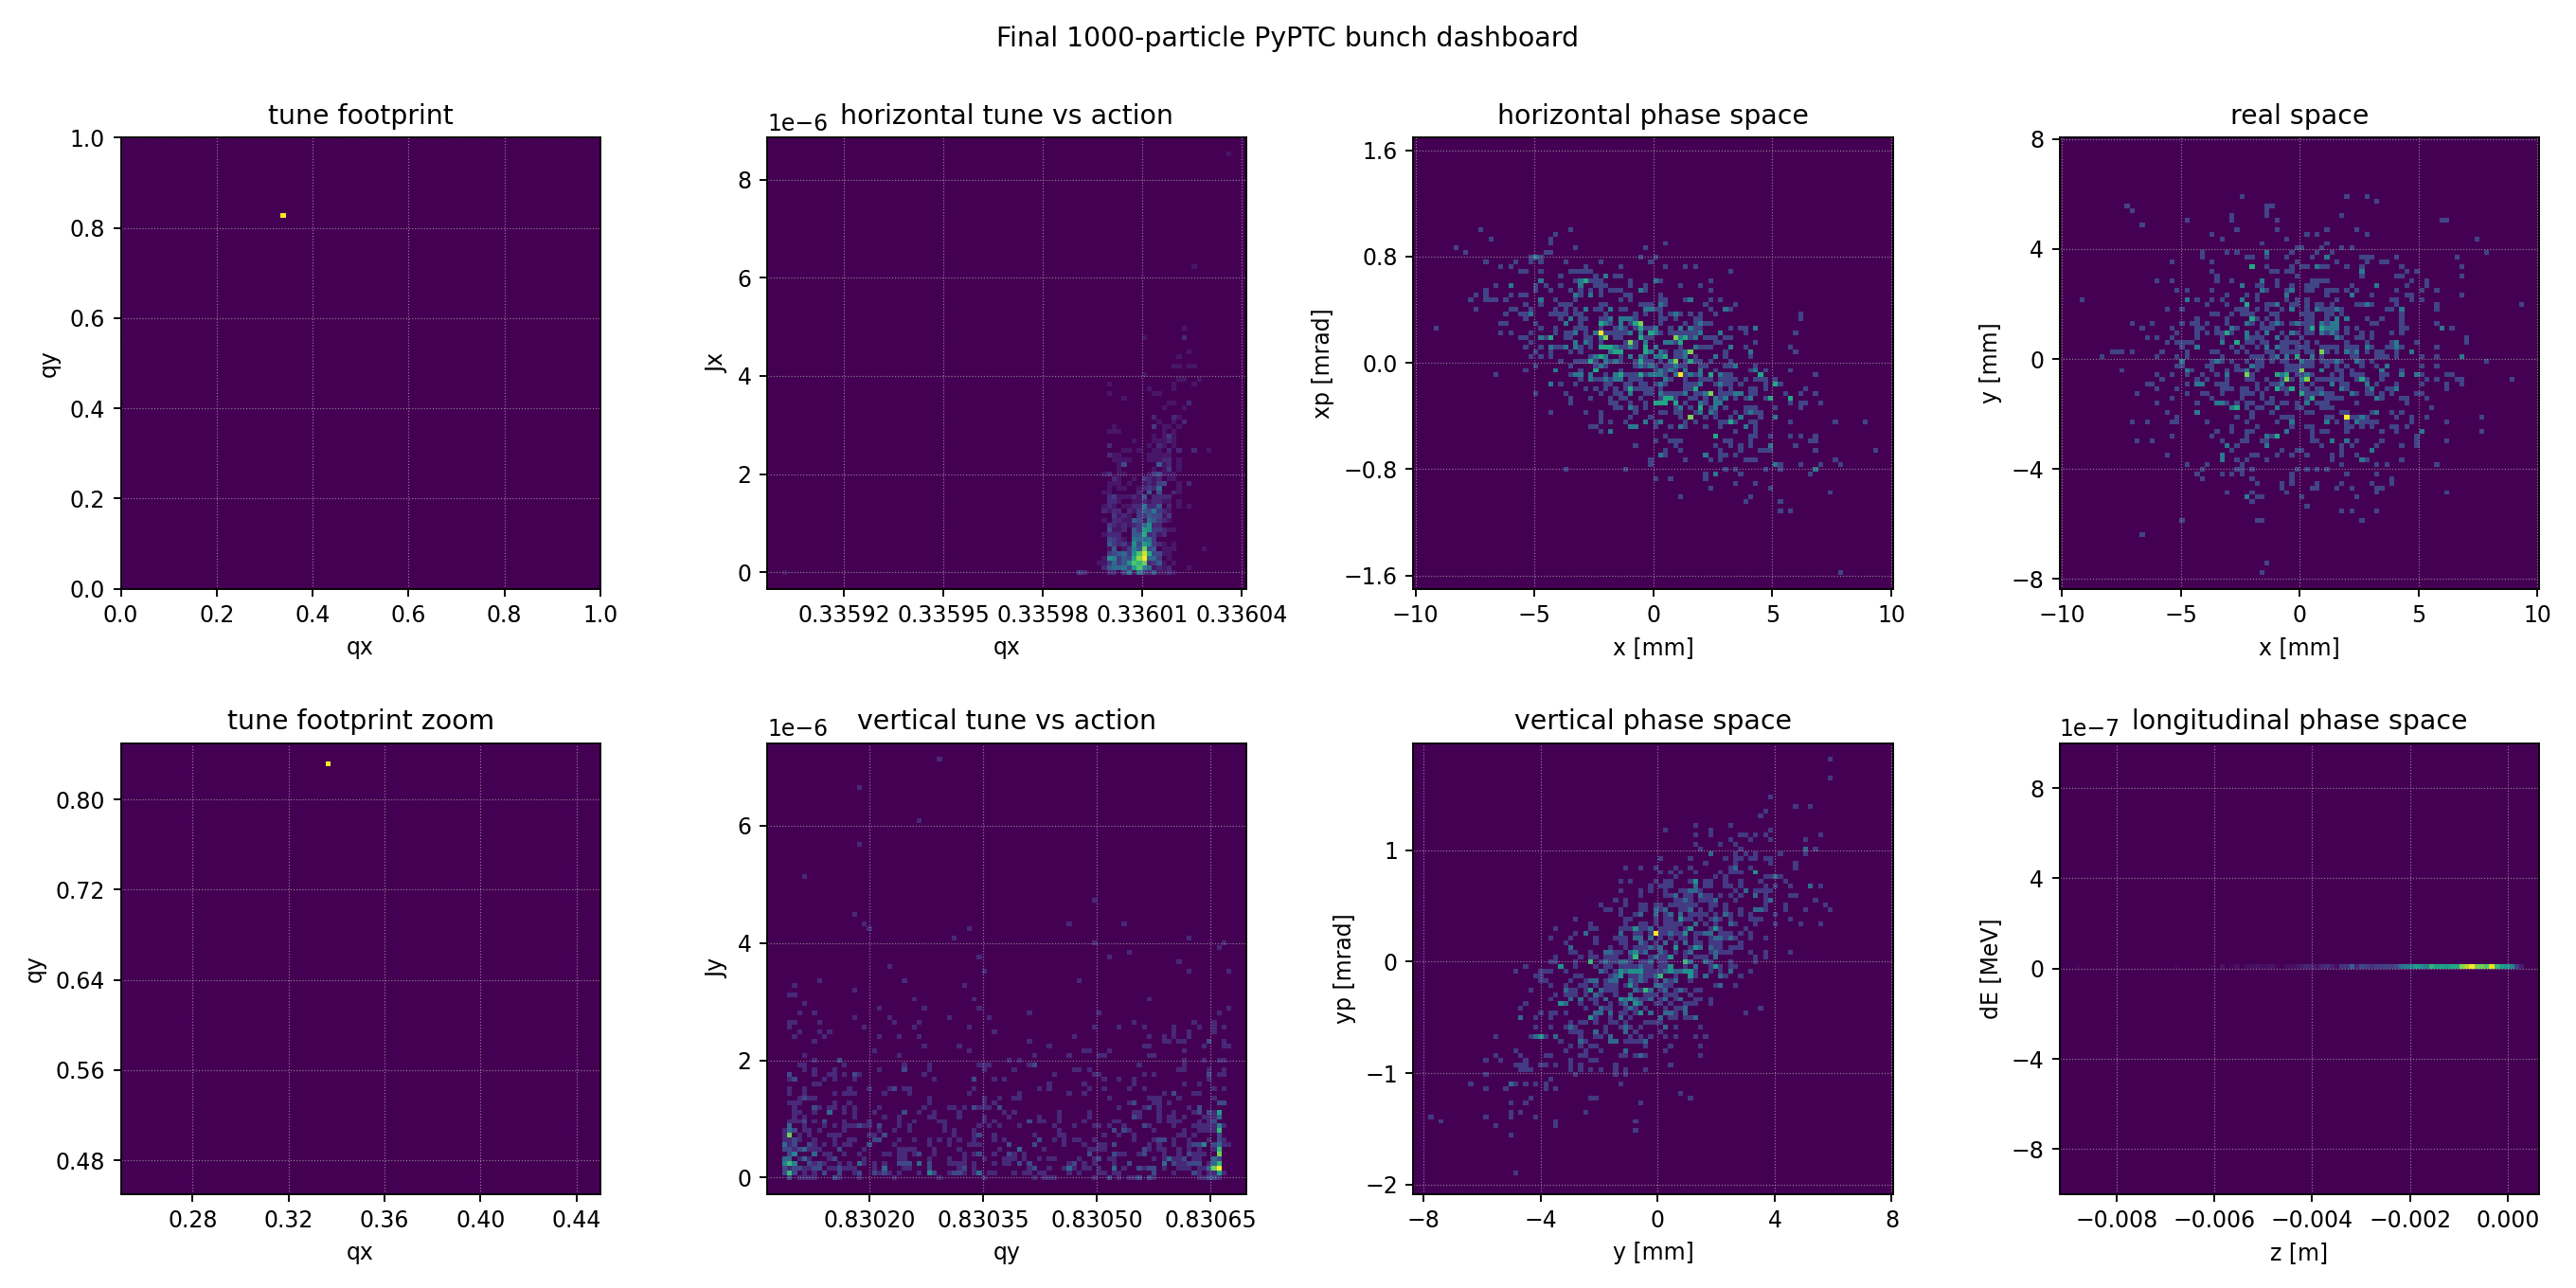
\includegraphics[width=0.88\textwidth]{figures/bunch_final_dashboard.png}
  \caption{Final bunch dashboard from the same example output. Its side-by-side interpretation is limited to this recorded run and the generated input bunch. [claim:PROV-03]}
\end{figure}

\subsection{Apertures and particle loss}

The aperture helpers read rectangular aperture assignments or TFS records, and the JVT CSV reader divides its semi-aperture columns by 1000 before constructing records. The API can apply, query, disable, and set absolute apertures; tracking returns loss flags and loss turn/position fields. The dimensions and operational meaning of input columns should be confirmed by the aperture data owner. [claim:AP-01]

\begin{figure}[ht]
  \centering
  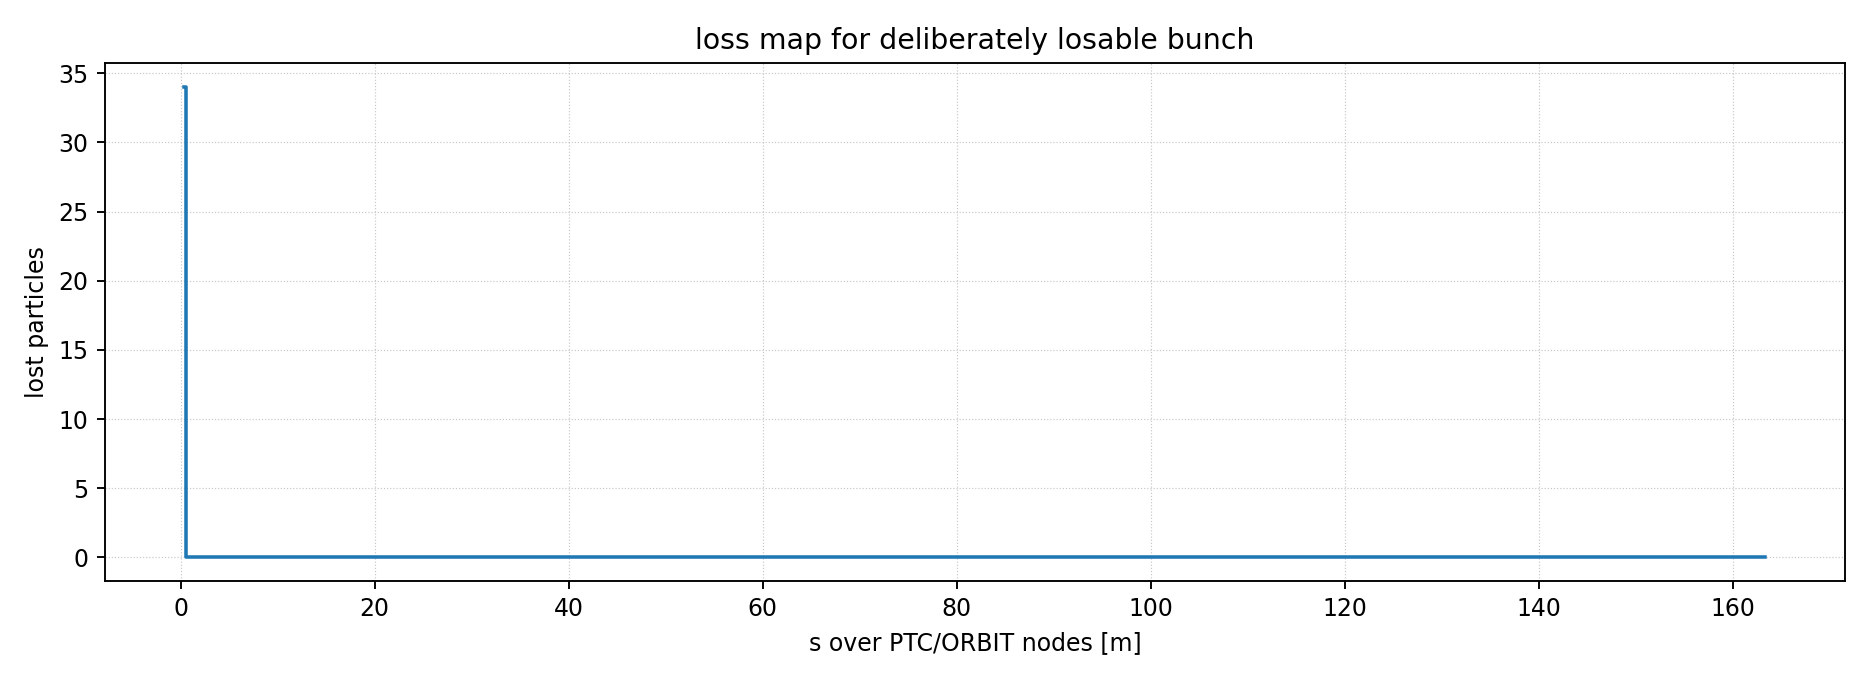
\includegraphics[width=0.82\textwidth]{figures/aperture_loss_map.png}
  \caption{Loss-map image from the aperture example output. It is an example visualization from the stored run and does not establish a validated physical aperture model. [claim:PROV-03] [claim:PROV-04]}
\end{figure}
